\subsection{Results and Discussion}
We collected 868 search entries with an average of 27 entries per person.
The average time taken to record a search activity was $131.6$ seconds ($median=120, max=1200$). 9\% of searches (33 out of 868) failed, not providing users with the information they sought. About a third (279 out of 868 search entries) were difficult (opposed to `easy' described below). 41.2\% used Google app, 49.4\% used a specific url, and the rest used other apps (i.e Amazon app). Participants performed an average of $1.2$ searches ($median=1, min =1, max=5$) and followed $2.5$ links ($median=2, min=0, max=39$) to find their information. Participants evaluated the task difficulty at an average of $1.9$ ($median=2,  stdev=1, min=1, max=5$) based on a Likert scale with 1 being very easy and 5 being very difficult. 

We looked for duplicate themes from collected diary entries and did not start with a set of fixed categories. We adopted most of the categories from \cite{chi2008} and added new categories such as `\emph{how-to}', `\emph{unit conversion}', `\emph{definition}', and `\emph{name}'. There are 17 categories based on the diary entries.
The \emph{how-to} category includes information about practical advice and detailed instruction of an activity. The \emph{unit conversion} includes kilometer to miles conversion, fahrenheit to celsius, and exchange rate. The \emph{definition} includes any need of terminology definition and detailed explanation. The \emph{name} includes search of a certain person or movie title. The largest category of collected entries was \emph{trivia} (51\%). They are the random thoughts from the participants such as ``story of shutter island". The second highest was \emph{shopping} (13\%), followed by \emph{point of interest} (10\%) and \emph{definition} (6\%).

We find several interesting discoveries from our study. People use applications more than websites for certain activities. On an average, 18.5\% (160 out of 868) of the searches were using applications than web portals. The most popular category searched using an application was \emph{shopping} (47\%). Surprisingly, participants frequently knew the exact keyword to put in as a search phrase. People use mobile apps for regular, standard search activities (i.e. weather, shopping, location, names, exchange rate, bus route, definition). For less frequent, more complicated searches, they will try it on a web portal but easily give up because of the screen size restriction and choose another method (i.e. go to their desktop, ask friends).

We divided searches into three categories beside success and fail. By collecting the number of keyword changes, the number of links, the time needed to finish a search, and the perceived difficulty rating, we measured the \emph{difficulty} level (easy/hard) of each search query. We define `easy' queries to be `at most one query made' and `perceived difficulty rating 3 or lower' and `open query or taken time lesser than 3 minutes'. Otherwise, a query is difficult.

We define open queries to be `two or more searches performed' or `information found does not fit into one typical webpage'. Open queries include broader subject-based explorations. Finally, we divided successful searches into hits or misses to reflect how hard users had to work to find their desired information. When users only had to follow one link, the search was a hit. 


Figure \ref{fig:searchtype} categorizes search type of diary entries by success/failure, easy/difficult, open/specific queries, and hit or miss. Overall, the large blue section shows that people are mostly successful in finding information with their mobile device (though they may never attempt many challenging searches). About a third of searches are still difficult, and over half of difficult searches are open. 


\begin{figure}[ht]
\centering
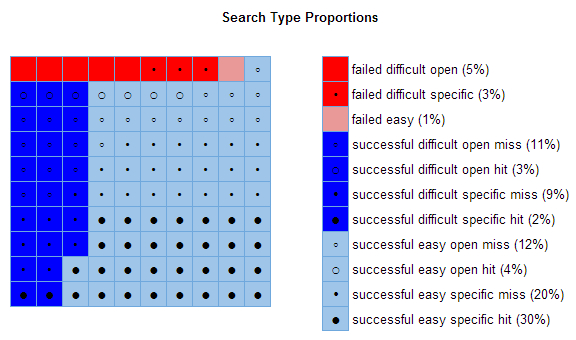
\includegraphics[width=3in]{images/searchtype}
\caption{Search type by success/failure, easy/difficult, open/specific, and hit/miss. Blue: success, red: failure, saturated color: easy, bright color: difficult, empty dot: open, filled dot: specific, smaller dot: miss, bigger dot: hit}
\label{fig:searchtype}
\end{figure}

Although search was usually successful, it was difficult about a third of the time, especially when search was more open and exploratory. Even among easy searches, over half were near misses requiring several clicks to find the needed information. In sum, we believe the large majority of searches could have benefited from a tool that helped users navigate through the information neighborhoods typical of open and near miss searches. 
